\chapter{Additional Tests}
\section{Effect of the BHA Size}
A sensitivity test was conducted to assess the impact of the BHA size on drill string vibration. For these simulations, exaggerated sizes of the BHA components were employed. The cases were based on Test Case 4 but different BHAs were used. Test Case 4b\_A1, Test Case 4b\_A2, and Test Case 4b\_A3 were run with the BHA's components outer diameter doubled, triple the length of the BHA, and both, respectively. \tablename~\ref{table_sensitivity_size_4b_input} summarizes the BHA properties for the tests.
\begin{table}
	\centering
	\begin{tabular}{|c|c|c|c|c|c|}
		\hline
        \tablecolumnheadervlinesone{Parameter} & \tablecolumnheadervlinestwo{Test Case 4b} & \tablecolumnheadervlinestwo{Test Case 4b\_A1} & \tablecolumnheadervlinestwo{Test Case 4b\_A2} & \tablecolumnheadervlinestwo{Test Case 4b\_A3} \\
		\hline
		$OD_{HWDP}$ & 0.1143 $m$ & 0.2286 $m$ & 0.1143 $m$ & 0.2286 $m$ \\
		\hline
		$ID_{HWDP}$ & 0.0635 $m$ & 0.0635 $m$ & 0.0635 $m$ & 0.0635 $m$ \\
		\hline
		$L_{HWDP}$ & 18.3 $m$ & 18.3 $m$ & 54.6 $m$ & 54.6 $m$ \\
		\hline
		$OD_{DC}$ & 0.1524 $m$ & 0.3048 $m$ & 0.1524 $m$ & 0.3048 $m$ \\
		\hline
		$ID_{DC}$ & 0.0508 $m$ & 0.0508 $m$ & 0.0508 $m$ & 0.0508 $m$ \\
		\hline
		$L_{DC}$ & 83.2 $m$ & 83.2 $m$ & 249.6 $m$ & 249.6 $m$ \\
		\hline
	\end{tabular}
	\caption[Input parameters for BHA size effect test for Test Case 4b]{Input parameters for BHA size effect test for Test Case 4b.}
	\label{table_sensitivity_size_4b_input}
\end{table}

The results presented in \figurename{}s~\ref{figure_AS_BHA_size_effect_vel} and \ref{figure_AS_BHA_size_effect_td} demonstrate the influence of the BHA size on the angular velocity and torque, respectively. Increasing the diameter of the BHA increased the maximum torque and decreased the frequency.  The increase in BHA length also increased the torque and decreased the vibration frequency.  Combining both changes to create a larger diameter and longer BHA amplified the effects further.

The larger diameter BHA increased the mass.  Because the mass was largely concentrated at the end of the string, it did not significantly change the overall stiffness.  This appreciably decreased the frequency of vibration.  It also increased the torque.  The increased mass required a larger force to accelerate it.  In addition, as this is a deviated well case, the increased mass also increased the friction forces and required more torque overcome them.

Lengthening the BHA added mass and reduced the stiffness.  The increased mass has all the same effects as mentioned in the previous paragraph.  The reduced stiffness decreased the frequency of vibration.

%It is observed that when the BHA length was increased (Test Case 4b versus Test Case 4b\_A2) a sudden increase in bit angular velocity occurred after the stick phase, while it originally occurred right before the stick phase. Moreover, the spikes of the bit velocity below 0 $RPM$ occurred when the BHA length was increased.

\begin{figure}
	\centering
	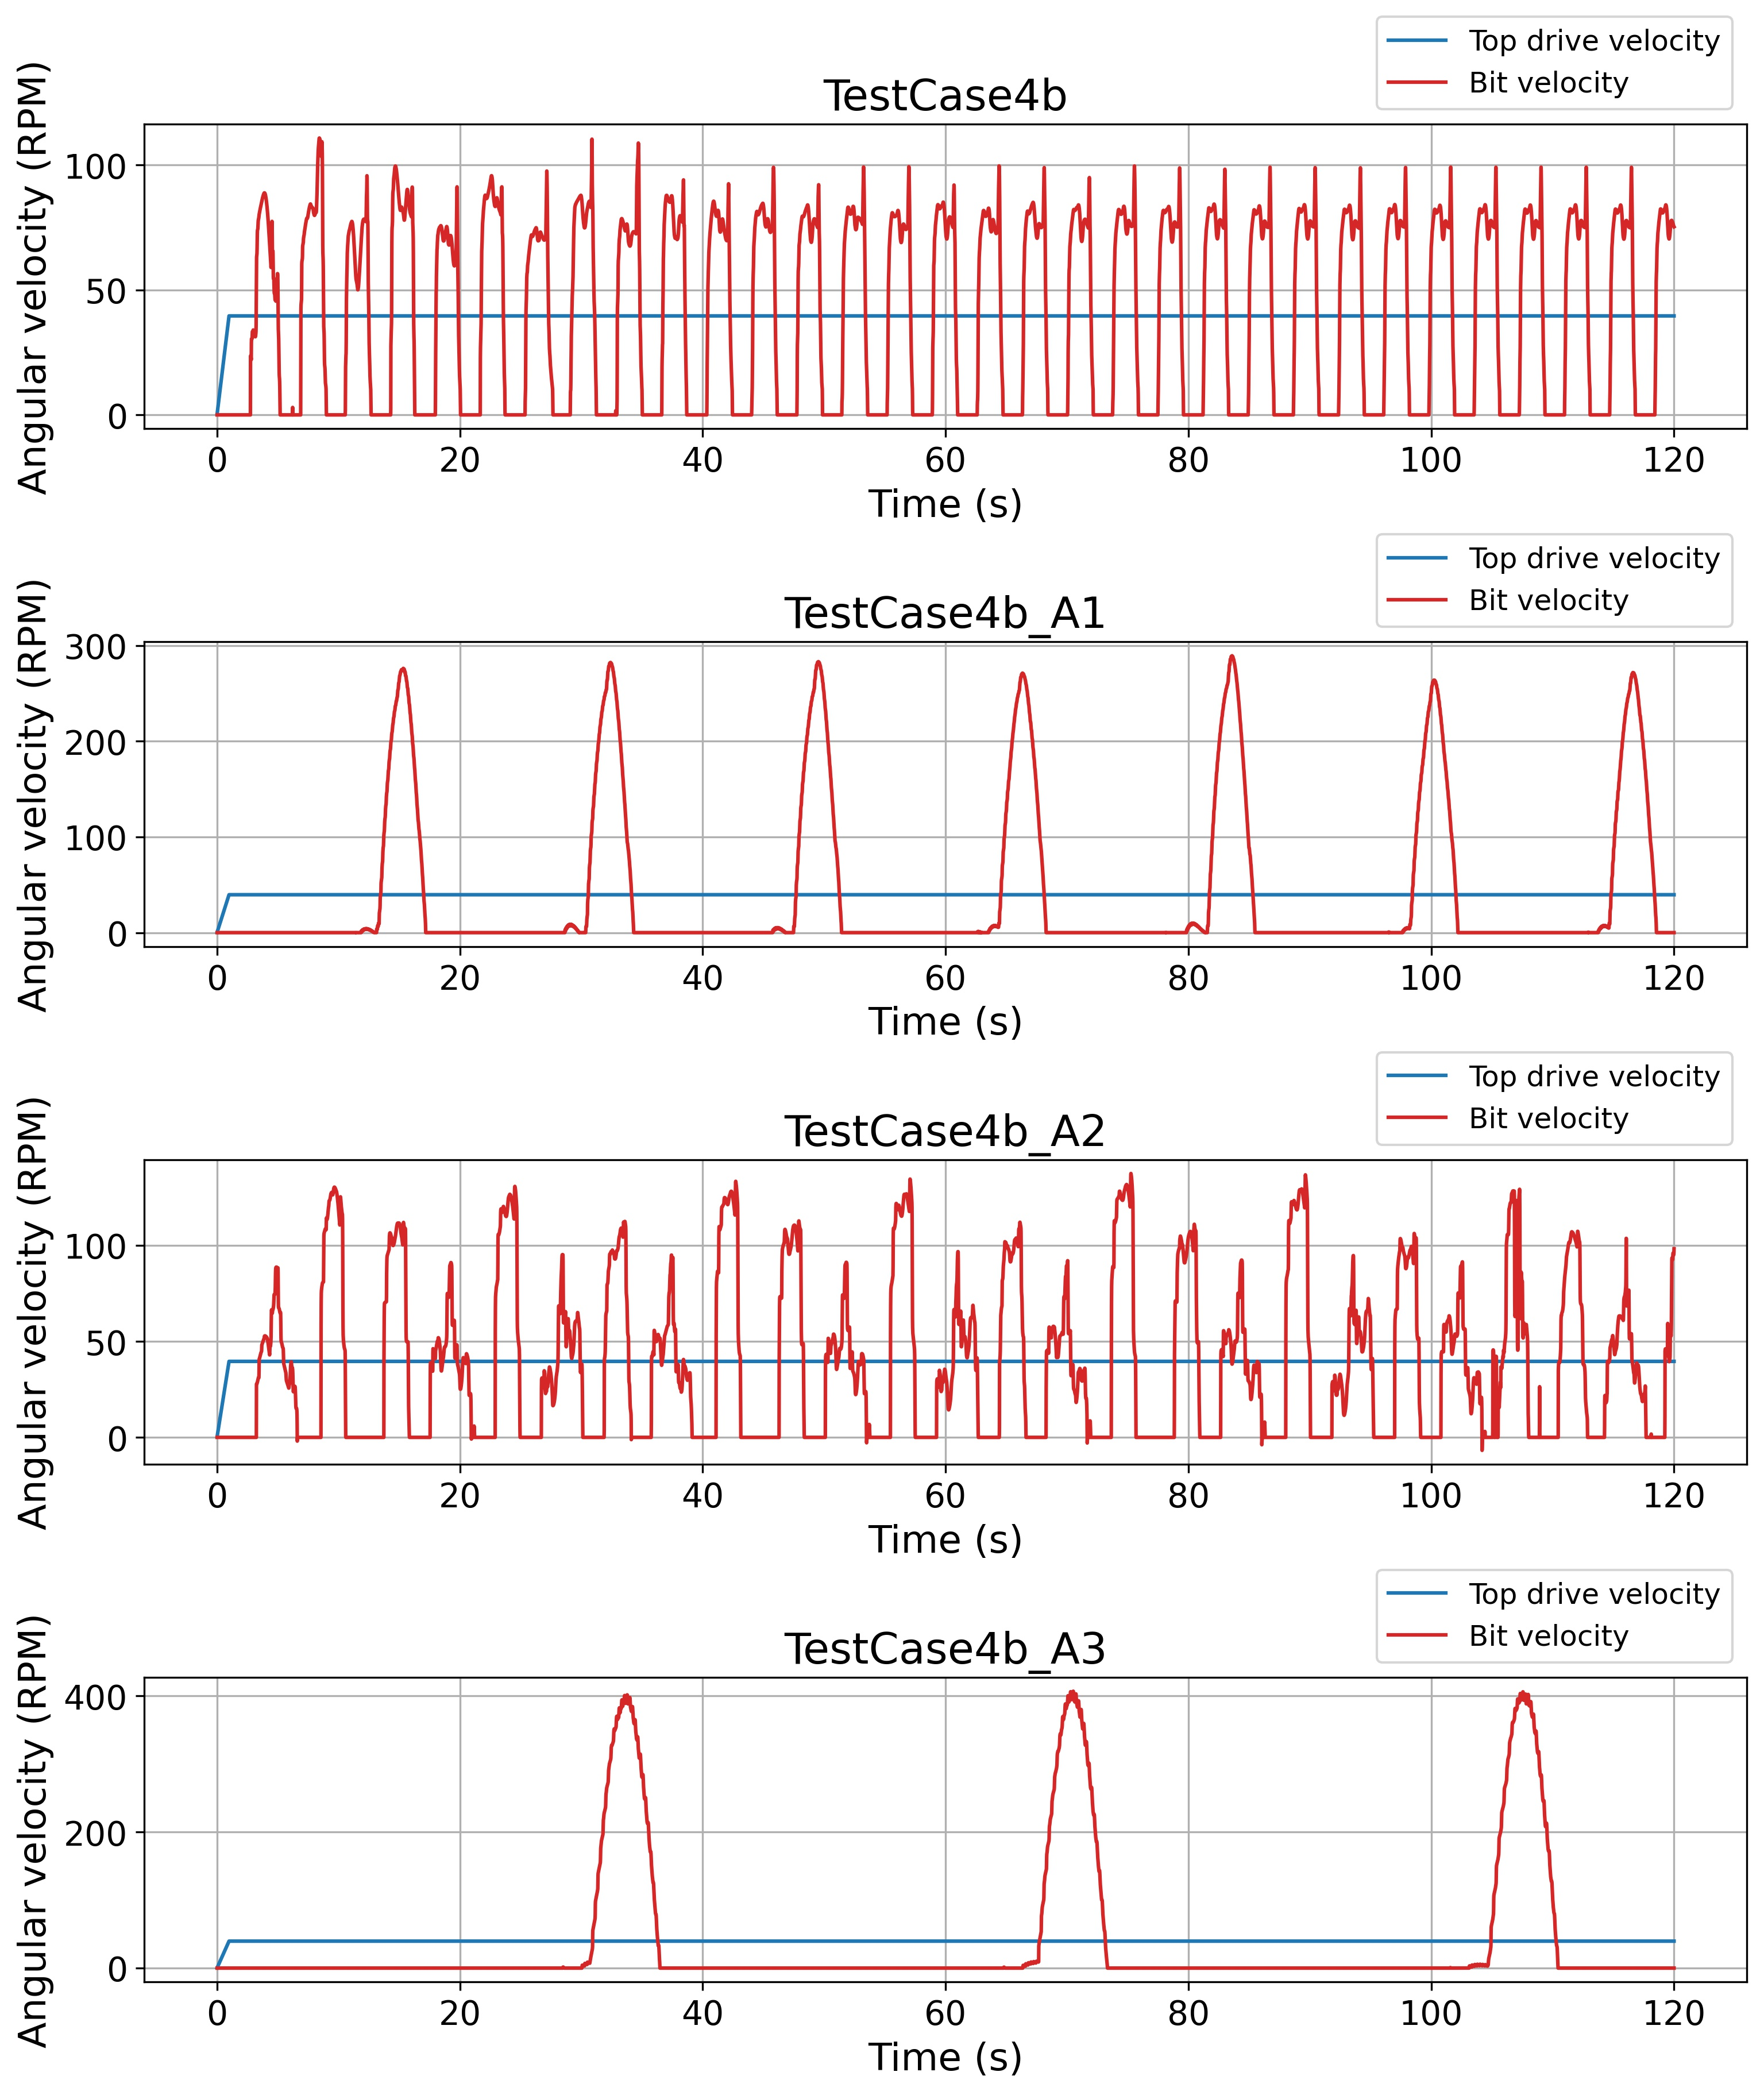
\includegraphics[width=\linewidth]{AS_size_effect_vel}
    \caption[Size effect of BHA components to angular velocity from A-S model]{Size effect of BHA components to angular velocity of bit from A-S model. The tests were conducted based on Test Case 4, where Test Case 4\_A1, Test Case 4\_A2 and Test Case 4\_A3 were simulated with doubled diameter, tripled length and both doubled diameter and tripled length of BHA components, respectively.}
	\label{figure_AS_BHA_size_effect_vel}
\end{figure}

\begin{figure}
	\centering
	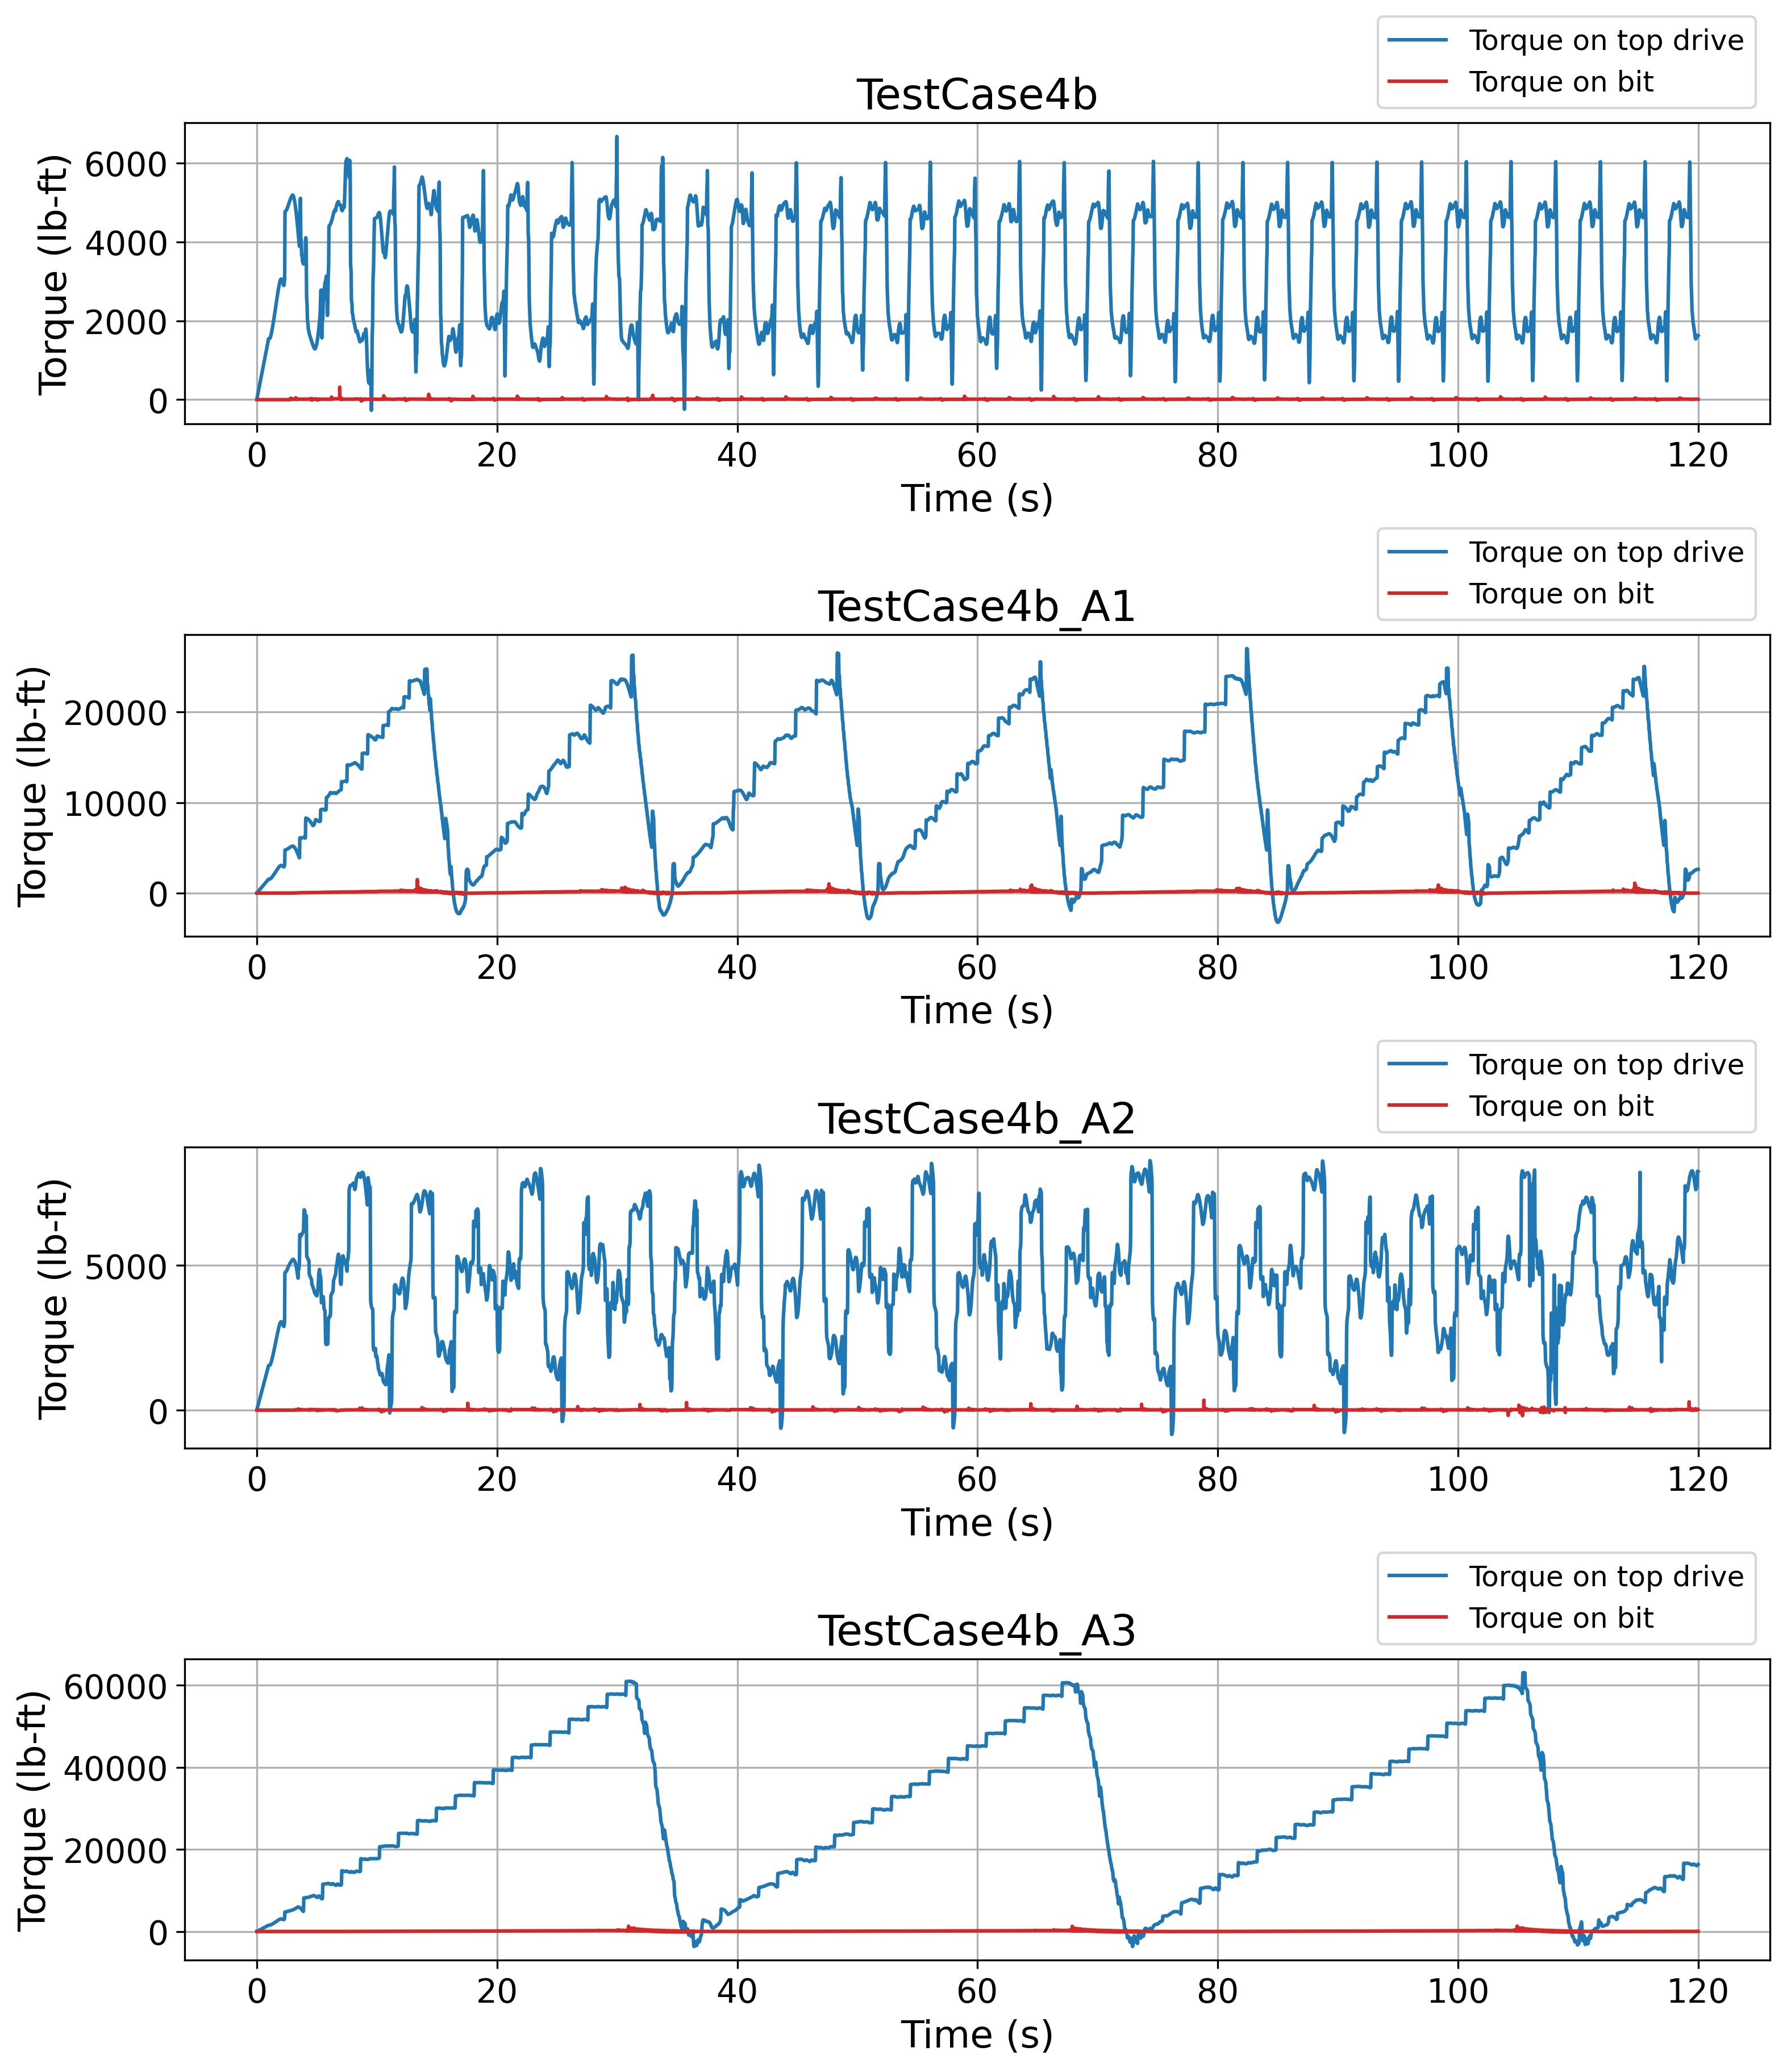
\includegraphics[width=\linewidth]{AS_size_effect_td}
    \caption[Size effect of BHA components to a torque from A-S model]{Size effect of BHA components to torque on top drive from A-S model. The tests were conducted based on Test Case 4, where Test Case 4\_A1, Test Case 4\_A2 and Test Case 4\_A3 were simulated with doubled diameter, tripled length and both doubled diameter and tripled length of BHA components, respectively.}
	\label{figure_AS_BHA_size_effect_td}
\end{figure}

%\section{Effect of Shear Modulus} 